\chapter{Heat equation -- 3D -- Temperature field of a solid object}

\modinfo{Directory}{TemperatureGeneric}
\modinfo{Solvers}{\Idx{HeatSolve}} 
\modinfo{Tools}{\Idx{ElmerGUI},\Idx{netgen},\Idx{OpenCascade}} 
\modinfo{Dimensions}{3D, Steady-state}
\modinfo{Author}{Peter R{\aa}back}


\subsection*{Problem description}

This tutorial tries to demonstrate how to solve the heat equation 
for a generic 3D object. The solid object 
(see figure~\ref{fg:object1}) is heated internally by a heat source.
\begin{figure}
\begin{center}
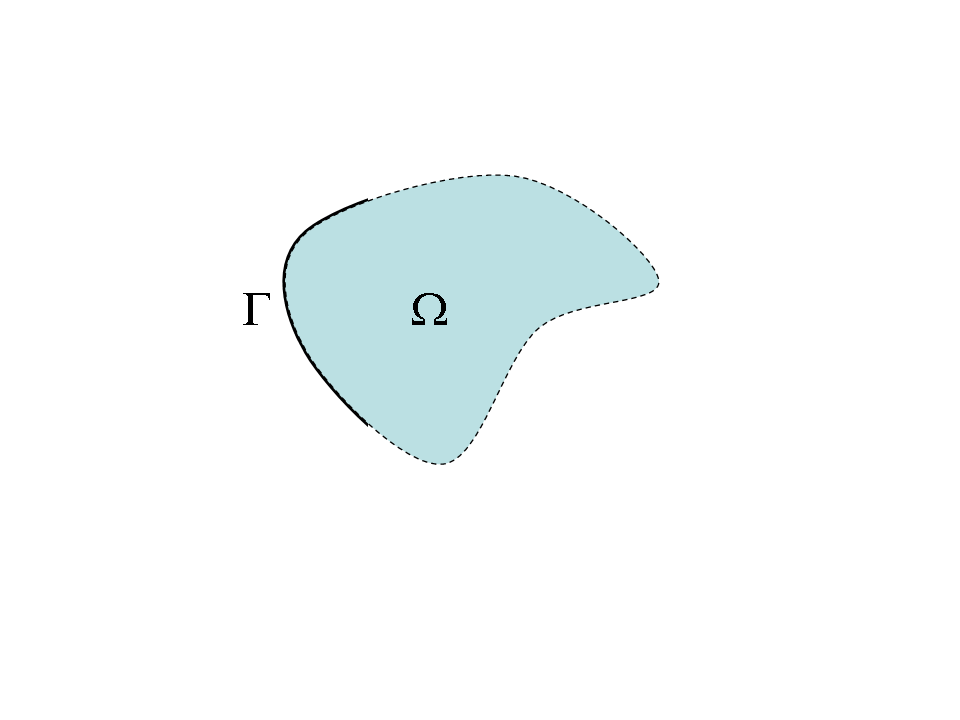
\includegraphics[width=80mm, viewport=100 100 760 520,clip]{domain}
\caption{Generic object being heated}\label{fg:object1}
\end{center}
\end{figure}
At some part of the boundary the temperature is fixed.
Mathematically the problem is described by the Poisson equation
\begin{equation}
\left \{
\begin{array}{ccccc}
- \kappa \Delta T &= &\rho f & \mathrm{ in } \, \, & \Omega \\
T&=&0 & \mathrm{ on } & \Gamma
\end{array}
\right .
\end{equation}
where $\kappa$ is the heat conductivity, $T$  is the temperature 
and $f$ is the heat source. It is assumed that density 
and heat conductivity are constants. 

To determine the problem we assume that the part of the boundary is fixed at $T_0=293$~K,
the internal heat generation is, $h=0.01$~W/kg, and use the material properties of aluminium.


\subsection*{Solution procedure}

Start \texttt{ElmerGUI} from command line or by clicking the icon in your desktop. Here we describe 
the essential steps in the ElmerGUI by writing out the clicking procedure. Tabulation generally means that the 
selections are done within the window chosen at the higher level. 

The geometry is given in step format in file \texttt{pump\_carter\_sup.stp}
in the \texttt{samples/step} directory of ElmerGUI, 
This file is kindly provided at the AIM@SHAPE Shape Repository by INRIA.
The heat equation is ideally suited for the finite element method and 
the solution may be found even at meshes that for some other problems
would not be feasible. Therefore you may easily experiment solving the same
problem with different meshes. If you lack OpenCascade you might try to solve a similar problem
with the \texttt{grd} files \texttt{angle3d.grd, angles3d.grd, 
bench.grd}, or \texttt{cooler.grd}, for example.

The CAD geometry defined by the step file is transformed on-the-fly by OpenCascade library into 
an stl file 
%may be used by both tetgen (tetlib) and netgen (nglib) mesh denerators to perform volume meshing. 
%In this tutorial we use tetgen.
for which nglib creates tetrahedral volume discretization.
You may also use the tetlib library (tetgen) if you have installed it as a plug-in.

Load the input file:
\ttbegin
File 
  Open -> pump_carter_sup.stp
\ttend
The meshing will take a minute or two. 
You should obtain your mesh and may check for the number of element in the \texttt{Model summary}. 
With netgen the default setting generates 8371 nodes and 36820 tetrahedral elements. 
Visual inspection reveals that the mesh is not quite satisfactory in geometric accuracy.
We choose to modify the mesh by altering the settings in the following way.
\ttbegin
View -> Cad model...
  Model -> Preferences...
    Restrict mesh size on surfaces by STL density = on
    Apply
Mesh -> Remesh
\ttend
The meshing operation takes a minute or two. 
The modified mesh should include 16159 nodes and 65689 tetrahedral elements
and be more appealing to the eye.
In order to affect the mesh density study the command-line options of the netgen manual.
Here we continue with the default mesh.

%The stl description of the mesh only provides with one body and one surface. 
%Therefore we need to divide the 
%existing surface. First choose the surface by clicking on it (it should turn red) and then 
%\ttbegin
%Mesh 
%  Divide Surface
%    Divide
%\ttend
%You may as well use the red icon with arrows pointing to different directions. 
%The algorithm separates all boundaries with more than 20 angle separation between surfaces.
We want to set the temperature at the inside of the holes and in that aim you may join the three boundaries (see figure~\ref{fg:bcs_chosen}).
For that aim we may choose the six pieces that constitute the boundaries as shown in the picture by pressing the \texttt{Ctrl}-key down.
\ttbegin
Mesh 
  Unify Surface
\ttend
\begin{figure}
\begin{center}
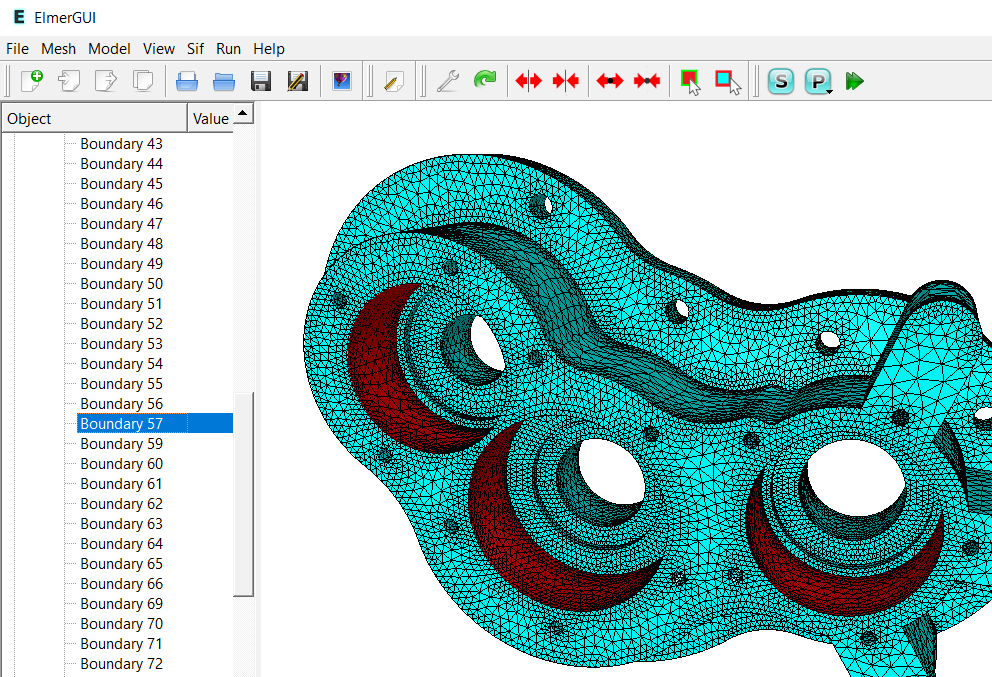
\includegraphics[width=100mm]{bcs_chosen}
\caption{The computational mesh showing the three joined boundaries}\label{fg:bcs_chosen}
\end{center}
\end{figure}

After we have the mesh we start to go through the Model menu from the top to bottom. 
In the \texttt{Setup} we choose things related to the whole simulation such as file names, 
time stepping, constants etc.
The simulation is carried out in 3-dimensional Cartesian
coordinates and in steady-state. 
Only one steady-state iteration is needed as the case is linear. 
\ttbegin
Model
  Setup 
    Simulation Type = Steady state
    Steady state max. iter = 1
\ttend
Choose \texttt{Apply} to close the window.

In the equation section we choose the relevant equations and parameters related to their solution. 
In this case we'll have one set only one equation -- the heat equation.

When defining Equations and Materials it is possible to assign to the bodies immediately, or to use mouse
selection to assign them later. In this case we have just one body and therefore it is easier to assign 
the Equation and Material to the body directly, whereas the active boundary is chosen graphically.

For the linear system solvers we are happy to use the defaults. One may however, try out different
preconditioners (ILU1,\ldots), for example.
\ttbegin
Model
  Equation
    Add 
      Name = Heat Equation
      Apply to bodies = Body 1
      Heat Equation
        Active = on
      Add   
      OK
\ttend        

The Material section includes all the material parameters.
They are divided to generic parameters which are direct properties of the material
without making any assumptions on the physical model, such as the mass. Other properties assume
a physical law, such heat conductivity.
We choose Aluminium from the Material library which automatically sets for the needed material properties. 
\ttbegin
Model
  Material
    Add 
      Material library
        Aluminium
      Apply to bodies = Body 1 
      Add 
      OK
\ttend

A Body Force represents the right-hand-side of a equation that in this case represents
the heat source. 
\ttbegin
Model
  Body Force
    Add 
      Name = Heating
      Heat Source = 0.01
      Apply to bodies = Body 1
      Add
      OK
\ttend    

No initial conditions are required in steady state case.

In this case we have only one boundary and set it to room temperature.
First we create the boundary condition
\ttbegin
Model
  BoundaryCondition
    Add 
      Heat Equation
        Temperature = 293.0
      Name = RoomTemp
      Add
      OK
\ttend   
Then we set the boundary properties 
\ttbegin
Model 
  Set boundary properties  
\ttend
Choose the defined group of three boundaries by clicking with the mouse
and apply the condition for this boundary.
\ttbegin
Boundary condition
  RoomTemp
\ttend

For the execution 
ElmerSolver needs the mesh files and the command file. We have now basically defined
all the information for ElmerGUI to write the command file. After writing it we may also visually 
inspect the command file.
\ttbegin
Sif 
  Generate
  Edit -> look how your command file came out  
\ttend

Before we can execute the solver we should save the files in a directory. In saving the project all the
necessary files for restarting the case will be saved to the 
destination directory.
\ttbegin
File 
  Save Project
\ttend

After we have successfully saved the files we may start the solver
\ttbegin
Run
  Start solver
\ttend
A convergence view automatically pops up showing relative changes of each iteration.
As the case is linear only one iteration was required for the solution and the second one
just is needed to check the convergence. The norm of the solution
should be around 432.4~K (with the default tetgen mesh 389.8~K, respectively).

Note: if you face problems in the solution phase and need to edit the setting, always remember to regenerate the
sif file and save the project before execution.


\subsection*{Postprocessing}

To view the results we use Paraview for the visualization,
\ttbegin
Run
  Paraview
\ttend
The default configuration shows just the object. To color the surface with the temperature choose the correct field.
The maximum temperature should be about 586.5~K.
You may turn on opacity in order to see through the object, 10-20\% is a good value.
This way you'll able to see some isosurfaces that you might want to define.
Some examples of the visualizations may be seen in figure~\ref{fg:vtkpost1}. Note that the pictures here
were generated by the obsolete VTKPost tool within ElmerGUI and therefore does not look like the
results in Paraview.

\begin{figure}
\begin{center}
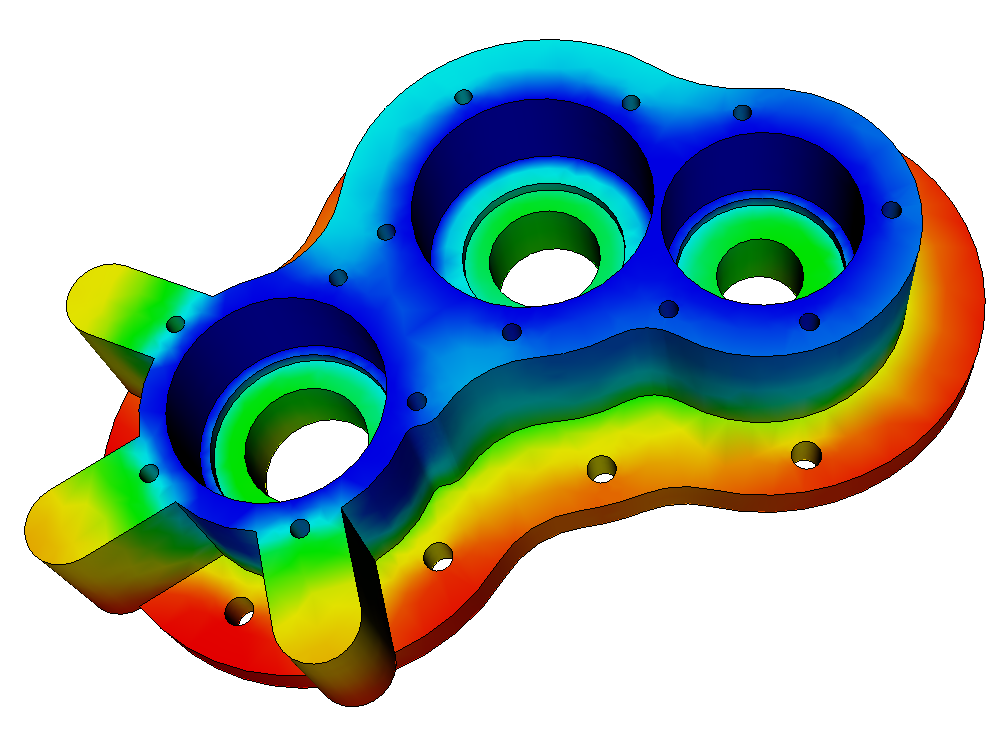
\includegraphics[width=120mm]{tempdist} \\
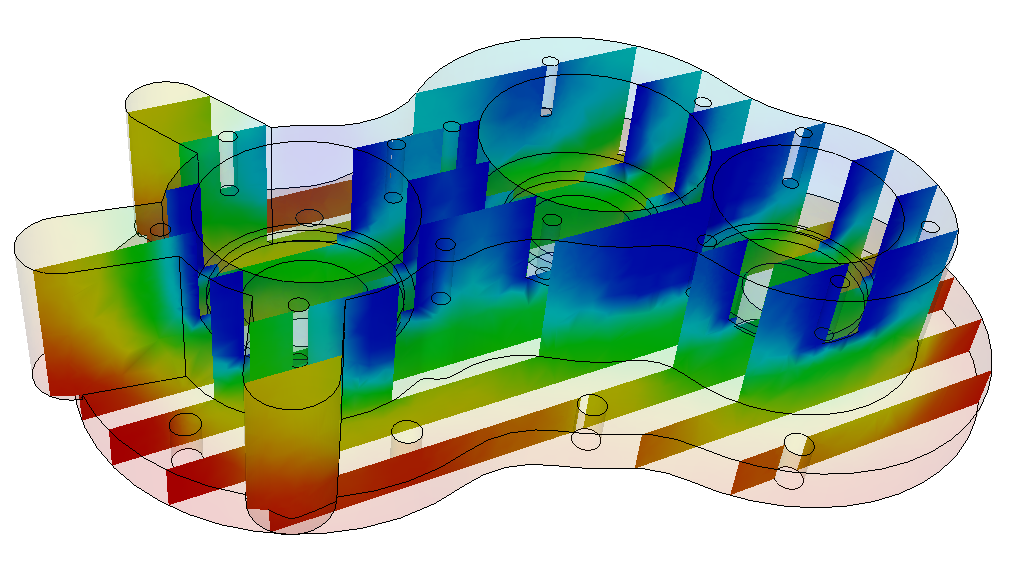
\includegraphics[width=120mm]{tempdist2}
\caption{The temperature distribution of the solid object domain.}\label{fg:vtkpost1}
\end{center}
\end{figure}

\hfill
\mbox{}






